\section{Tooling}
As mentioned in Section~\ref{eth:evm}, Ethereum offers a code execution
environment via the Ethereum Virtual Machine. The EVM is responsible for
executing a set of low-level instructions which can be used to update the state
of the network.\cite{ethereum-yellow} A number of higher-level languages exist
that are capable of being compiled into the low-level bytecode representation
required by the EVM for execution; this research uses the Solidity language. In
order for the EVM to execute bytecode, it must first exist on the Ethereum
blockchain. Deployment of bytecode to the Ethereum blockchain is performed by
constructing, and submitting to the Ethereum network, an account creation
transaction which includes the EVM bytecode. The account creation transaction
instructs the EVM to create a new account and to store the included bytecode
within it. Upon receiving the account creation transaction the EVM will execute
a special {\tiny{CREATE}} instruction (see Table~\ref{tab:gas-costs}) which
will eventually result in the creation of an ``internal account.'' This
internal account will contain the EVM bytecode, submitted with the create
account transaction, and is commonly referred to as a ``smart contract.'' Once
a smart contract exists on Ethereum blockchain, the bytecode stored within it
can be executed by constructing and submitting another transaction to the
network; this time instructing the EVM to execute the bytecode stored within
the smart contract. Beyond the bytecode stored in them when created, smart
contracts also contain and maintain their own internal state on the network,
which they can use as storage.

\subsection{Frameworks}
Given the complex process involved in compiling and deploying smart contracts to
the Ethereum network, a framework is typically leveraged to simplify development
and manage the smart contract deployment life-cycle. This research leveraged two
different software frameworks to aid in the development of smart contracts:
Embark and Truffle. Both of these frameworks aid in the compilation of Solidity
code, deployment of EVM bytecode, provisioning of test networks, and testing of
contract functionality.

\subsubsection{Embark}
Initially, smart contract implementations were built using the Embark framework.
The Embark framework is designed to aid in the construction and deployment of
Decentralized Applications (DApps); it supports functionality to provision test
networks, build and deploy contract code, and execute tests against deployed
smart contracts. The Embark framework is capable of managing, and deploying
contracts to, various other Ethereum blockchains; e.g., the testnet, private
net, and livenet. The Embark framework supports several useful development
features. For example, Embark can be configured to detect changes to contract
code during development, then trigger a recompilation and redeployment of
modified contract code to the appropriate Ethereum networks.

To build Solidity code into EVM bytecode, the Embark framework leverages
\solt{solcjs}, which offers JavaScript bindings for the Solidity compiler. For
expedited development and testing, Embark exposes the Ethereum JavaScript
\solt{testrpc}. The \solt{testrpc} simulates a fully functioning Ethereum
client, features an API for programmatic interaction (a useful feature during
test execution), and is capable of transaction execution speeds that complete
near-instantaneously (speeds which could not be matched by a live Ethereum
network). Embark simplifies interaction with Ethereum contracts by generating
contract-equivalent (promise-based) JavaScript functions that can be called to
execute contract code. JavaScript support is provided by wrapping the
\solt{web3js} library which implements the generic Ethereum JSON RPC spec.

The Embark framework also boasts support for other tools useful for building
decentralized applications; decentralized storage support via IPFS,
decentralized messaging functionality via Whisper and Orbit, and a curses-like
dashboard which exposes logs, environment configuration, contract state, service
availability, the status of application components and dependencies, and
features an interactive console for executing commands and querying application
state. A screenshot of the Embark dashboard is shown in
Figure~\ref{fig:embark-dashboard}.

\begin{figure}[H]
  \centering
  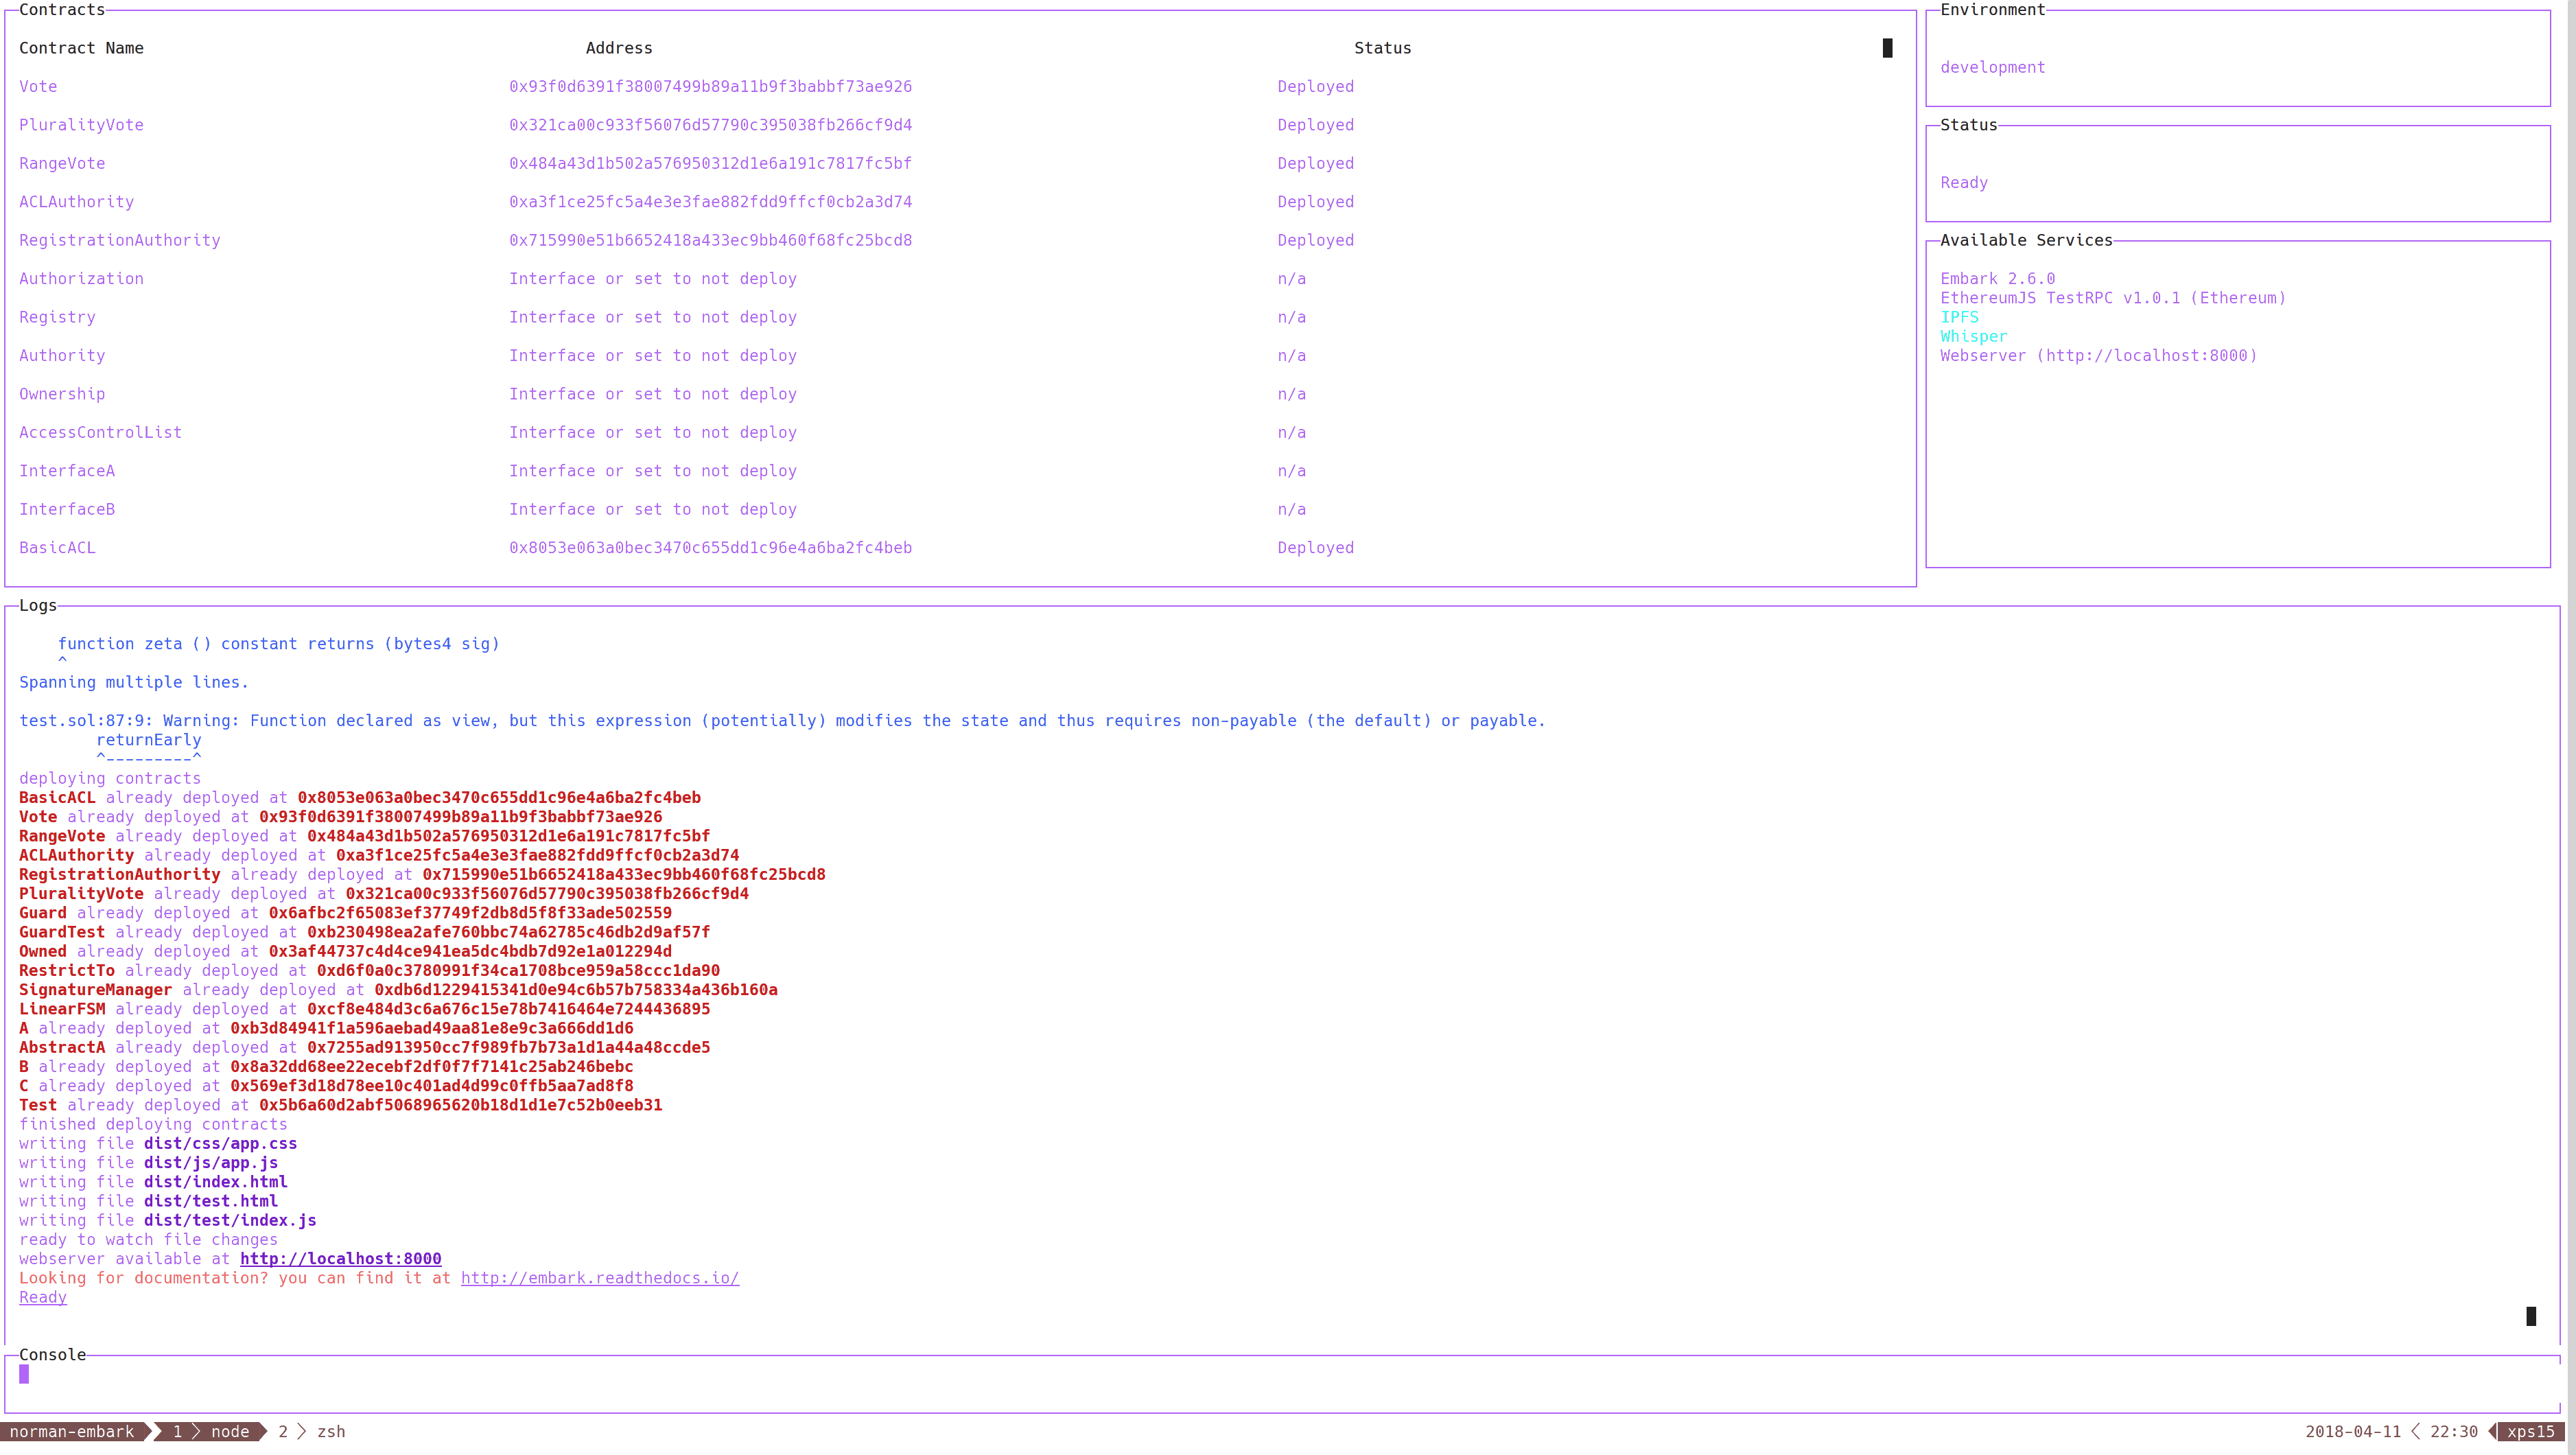
\includegraphics[width=\textwidth]{embark-ui-transparent-bg}
  \caption{The Embark dashboard and application state.}\label{fig:embark-dashboard}
\end{figure}


\subsubsection{Truffle}
Later smart contract development was completed using the Truffle framework. When
compared to the contract development features of the Embark Framework, the
Truffle framework can be viewed as an almost feature-identical framework ---
i.e., smart contract lifecycle management, testing functionality, JavaScript
bindings, and network management --- however, unlike the Embark framework, the
Truffle framework offers essentially no features related to DApp development.
The Truffle framework's more targeted focus with regards to smart contract
development and management produced a cleaner development experience during the
pursuit of this research, which is concerned strictly with smart contract design
and implementation and not DApp development. Furthermore, the Truffle framework
supports executing workflows and tests in TypeScript, and can be used in
conjunction with \solt{TypeChain} to generate TypeScript types for use with the
smart contract bindings generated by Truffle. A screenshot displaying the
execution of a contract test via the Truffle framework can be seen in
Figure~\ref{fig:truffle-test}.

\begin{figure}[H]
  \centering
  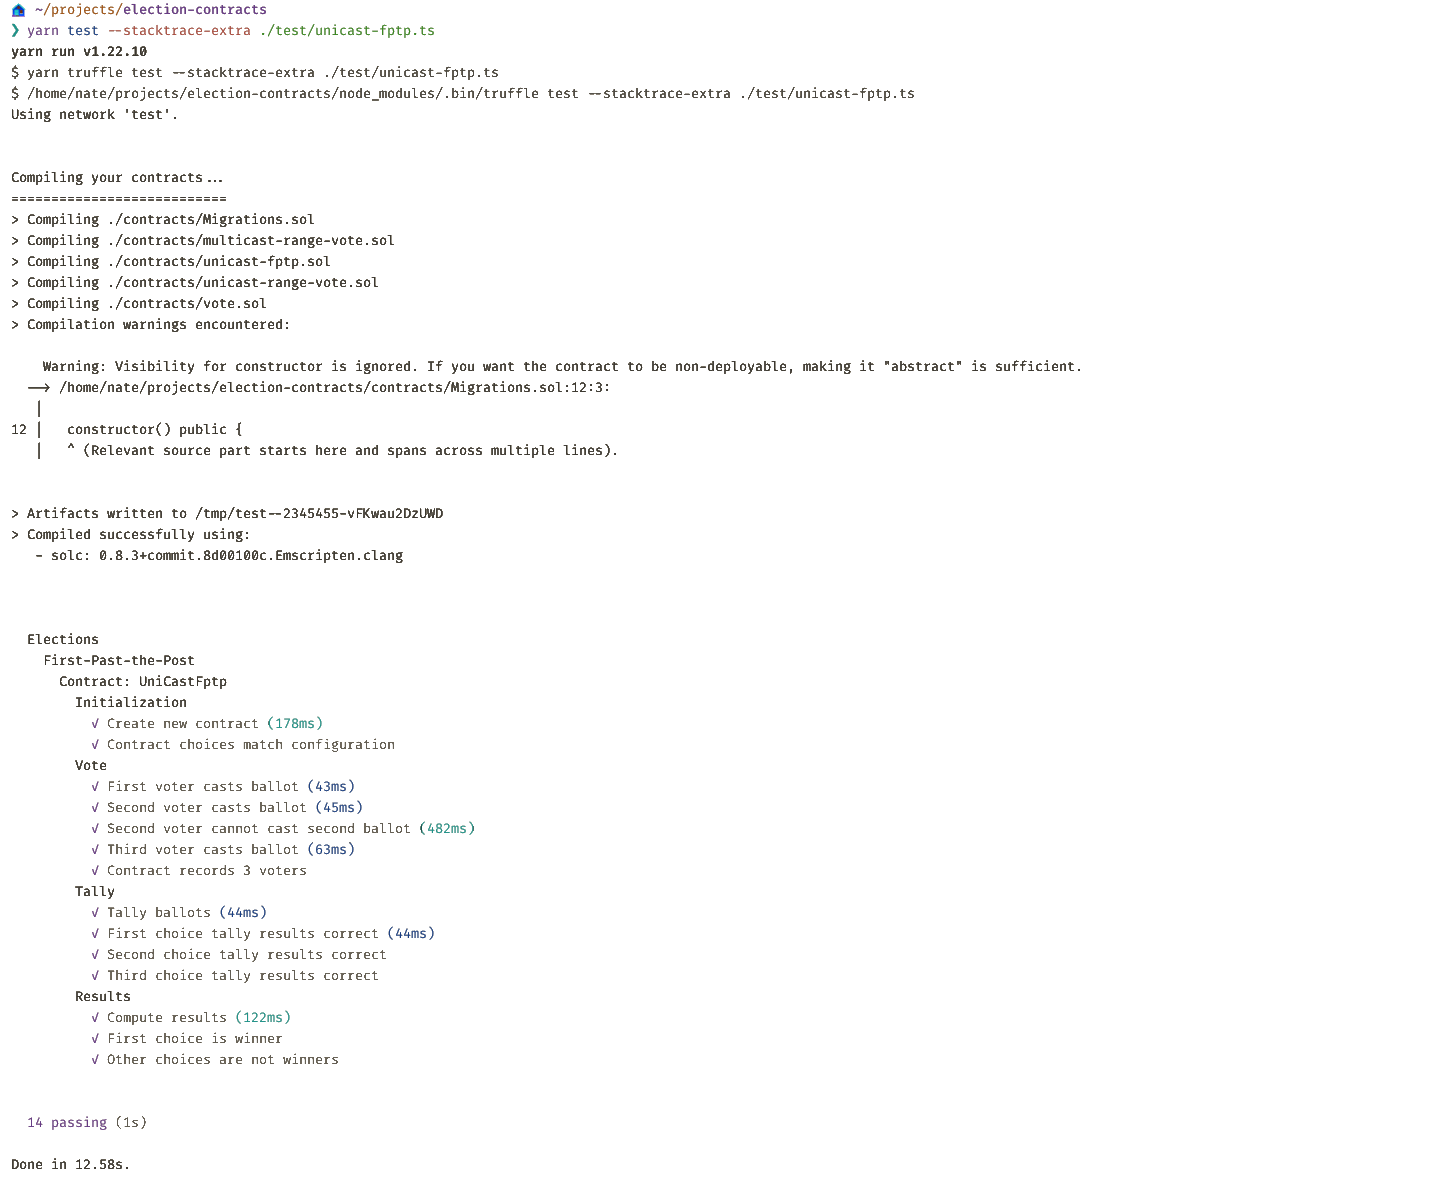
\includegraphics[width=\textwidth]{truffle-test-transparent-bg}
  \caption{Testing an election contract using the Truffle framework.}\label{fig:truffle-test}
\end{figure}

% seemed to result in to  i.e., lifecycle management, contract testing and
% debugging,
